% (c) 2020 Stefan Antonowicz
% Based off of tex found at https://github.com/ludus-leonis/nipajin
% This file is released under Creative Commons Attribution-NonCommercial-ShareAlike 4.0 International License.
% Please do not apply other licenses one-way.

\renewcommand{\yggMiscellania}{%
  \mychapter{Miscellany}{miscellany}
}

\renewcommand{\yggMiscellaniaText}{%

  \mysection{Effects}{effects}


  \mysubsection{Afraid}{effect-afraid}

  If you are Afraid of something, you must \RS : Sanity when you approach or attack the object of your fear.  Remember, if you fail a \RS : Sanity, you must roll on the \mylink{Terrifying Tables}{misc-terrifying-tables}

  If you damage the object of your Fear, the Fear is immediately dispelled

  If a Monster is a Afraid of something, it will try to run away.  If left to its own devices it will hide in the adjacent room / area that is most safe and return when the duration is up.  Monsters resist Fear with a morale check.

  \mysubsection{Anathema}{effect-anathema}

  You cannot benefit from magical healing or be the target of helpful magic (note: Leechcraft isn't magical healing).  You automatically fail any Saves against Hexes, and you cannot gain Glory through Carousing.

  \mysubsection{Befuddled}{effect-befuddled}

  If you are Befuddled, you cannot tell any two creatures apart - everyone looks the same. Whenever you attack, you attack a random creature.  When you cast a spell, you cast a random spell at a target picked randomly from all eligible ones.  Whenever you try to run through a door, you run through a random door.  The Arbiter should feel free to dictate additional effects as necessary.

  \mysubsection{Bleeding}{effect-bleeding}

  If you are Bleeding, you lose 1 Flesh every Moment.  This doesn't stack (i.e. you can't Bleed for 2 damage every Moment).

  \mysubsection{Blinded}{effect-blinded}

  You can't see.  You automatically fail \RO checks, Init rolls, and any other skills that require sight.

  \mysubsection{Charmed}{effect-charmed}

  You treat the person who Charmed you like a good friend, and ignore the obvious spell they just cast on you.

  \mysubsection{Concussed}{effect-concussed}

  You automatically lose Init and any Skill or Saves rolls take a -4 penalty

  \mysubsection{Deafened}{effect-deafened}

  You can't hear.  You automatically fail Listen checks, Init rolls, and any other skills that require hearing.

  \mysubsection{Disgusted}{effect-disgusted}

  You fight through your feelings of revulsion or horror, but all \RO, \RB, or \RS have a -4 modifier as long as you are in the presence of the object of your disgust.

  \mysubsection{Disarmed}{effect-disarmed}

  Can only affect things held in one hand (like 1h weapons). The item is ripped from your grasp and falls to the ground.  It will take an Action to recover it.

  \mysubsection{Drunk}{effect-drunk}

  You get a -1 on all \RO tries for every point of Drunk (up to a -4).  When you Bivouac, roll a \RS : \VIG.  If you fail, you are Hung Over at the end of the Bivouac.

  \mysubsection{Enraged}{effect-enraged}

  You immediately attack whatever has afflicted you. While in a rage, you have +4 Fight modifier, deal +4 Damage, and are immune to Fear. While raging, you cannot do anything defensive, curative, tactical, or cooperate with your allies. If the object of your rage isn't a living thing, you will destroy it any way you can. Spellcasting is impossible.  You cannot stop fighting until you destroy the object or all Monsters are dead.  If an Ally hurts you during your rage, they are considered a Monster.

  \mysubsection{Hung Over}{effect-hung-over}

  Roll a d4.  1) You are at -4 on all \RO tries;  2) You are \mylink{Sickened}{effect-sickened};  3) You are \mylink{Concussed}{effect-concussed}; 4) You are \mylink{Woozy}{effect-woozy}.  The effect lasts until it is a) removed by Leechcraft, or b) removed with an appropriate tonic (Chymistry) or narcotic, or c) you Bivouac, or d) you acquire enough point of Drunk to equal what you rolled on the d4.


  \mysubsection{Invisible}{effect-invisible}

  You cannot be seen as long as you don't move.  If you're invisible, you can see other invisible objects.

  \mysubsection{Knocked Out}{effect-knocked-out}

  You immediately drop Prone and drop any items you're holding.  Fight rolls against you hit automatically, bypass Grit, do maximum damage (Crit) and can only be blocked by Armor.  If the effect is not Markovian, roll a \RS : \VIG at the top of each Moment; if you succeed, you awaken (but you are still Prone).  Once you awaken, the effect ends.

  \mysubsection{Paralyzed}{effect-paralyzed}

  You immediately grow rigid - you cannot move or act, even to defend yourself.  Guard rolls automatically fail: the attack bypasses Grit, does maximum damage (Crit) and can only be blocked by Armor.  

  \mysubsection{Prone}{effect-prone}

  If you are knocked Prone you must spend an action getting to your feet.  While you are in a prone position you can continue to Fight and Guard at a -4 penalty

  \mysubsection{Shaken}{effect-shaken}

  Synonymous with Disgusted, but usually occurs from something that terrifies you.

  \mysubsection{Shocked}{effect-shocked}

  Immediately drop anything you're holding.  If you are shocked as the result of a Horror you have witnessed, your hair turns snow white.

  \mysubsection{Sickened}{effect-sickened}

  You are overcome with nausea and being vomiting, dry-heaving, etc.  You cannot Fight and can only Guard at a -4.

  \mysubsection{The Vapors}{effect-the-vapors}

  You immediately pass out.  Any damage will wake you up immediately, but any attacks against you bypass Grit, do maximum damage (Crit) and can only be blocked by Armor.

  \mysubsection{Woozy}{effect-woozy}

  You take a -4 penalty to \myital{every} \RO  and \RB  attempt (including Fight and Guard)


  \mysection{Vision}{vision}

  \mysubsection{Dark Sight}{vision-dark-sight}   

  You can see in complete, utter darkness with no hindrance.  If you have Dark Vision you take a -4 on tries and attacks involving sight, done in daylight (or similar levels), that are further away than Close. 

  \mysubsection{Day Vision}{vision-day-vision}

  You see in daylight but take a -4 on tries and attacks in darkness for any test involving sight that is further away than Close. 

  \mysubsection{Low Light Vision}{vision-low-light-vision} 

  You can see in normal daylight and in dim lit conditions like starlight with no hindrance. In darkness, however, you must roll -4 on tries and attacks involving sight that are further away than Nearby.


  \mysection{Terror, Horror, and Madness}{terror-horror-madness}
   
  \myital{This is taken almost verbatim from \href{https://talesofthegrotesqueanddungeonesque.blogspot.com}{"Tales of the Grotesque and Dungeonesque"}}

  In Gothic literature, the experience of terror is frequently described as a soul-expanding experience of awe. When one feels terror, one's mind is elevated to a new understanding of the world's terrifying possibilities; possibilities that were once repressed by the rational mind now threaten to undue the psyche's defenses. As such, terror is generally an inward experience; it is centered on psychological interiority, the ways in which a sense of self is located in relation to the outside world, and the realization of our inconsequential smallness in the face of something unthinkable.

  In many ways, the experience of horror is the opposite of the experience of terror; feelings of horror are soul-shrinking impressions of disgust or revulsion. When one feels horror, one's mind contracts and attempts to shut out the horrifying possibilities of what you've just experienced or attempts to repress the horrible implications of what you've just witnessed. In Gothic literature, objects that inspire horror are generally exterior to the sense of self; they are more visceral than actively psychological.

  \mysubsection{Terrifying Tables}{misc-terrifying-tables}

  Depending on whether the character is affected by Terror or Horror, roll on the appropriate table below.  If they roll a 6 (Madness!), roll a d20 on the Madness chart.  Any effects other than Madness lasts until you Bivouac. Madness can only be cured by a Leech during a Vacation, or by a wisewoman or doctor in a Sanitarium. 

  \cbreak

  \mysubsection{Terror}{misc-terror-table}


  \mytable{X c }{
    \thead{d6} & \thead{Result} \\
  }{
    1 & \mylink{Shaken}{effect-shaken} \\
    2 & \mylink{Woozy}{effect-woozy} \\
    3 & \mylink{The Vapors}{effect-the-vapors} \\
    4 & \mylink{Afraid}{effect-afraid} \\
    5 & \mylink{Paralyzed}{effect-paralyzed} \\
    6 & \mylink{Madness!}{misc-madness-table} \\
}

  \mysubsection{Horror}{misc-horror-table}

  \mytable{X c }{
    \thead{d6} & \thead{Result} \\
  }{
    1 & \mylink{Disgusted}{effect-disgusted} \\
    2 & \mylink{Shocked}{effect-shocked} \\
    3 & \mylink{Sickened}{effect-sickened} \\
    4 & \mylink{Afraid}{effect-afraid} \\
    5 & \mylink{Enraged}{effect-enraged} \\
    6 & \mylink{Madness!}{misc-madness-table} \\
}

  \mysubsection{Madness!}{misc-madness-table}

  \mytable{X c }{
    \thead{d20} & \thead{Result} \\
  }{
    1  & The Needle \\
    2  & Melancholy \\
    3  & Darkfear \\
    4  & Whisper of the Rapture \\
    5  & Amnesia \\
    6  & Occult Obsession \\
    7  & Gluttony \\
    8  & Occult Obsession \\
    9 & Foolhardiness \\
    10  & Blind Fury \\
   11  & Shot Nerves \\
   12  & Odious Quirk \\
   13  & Night Terrors \\
   14 & Fanaticism \\
    15  & Hallucinations \\
    16  & Starvation \\
    17  & Beaten \\
    18  & Split Personality \\
    19 & The Voices \\
    20  & True Madness \\
  }


  \newpage

  \begin{center}
  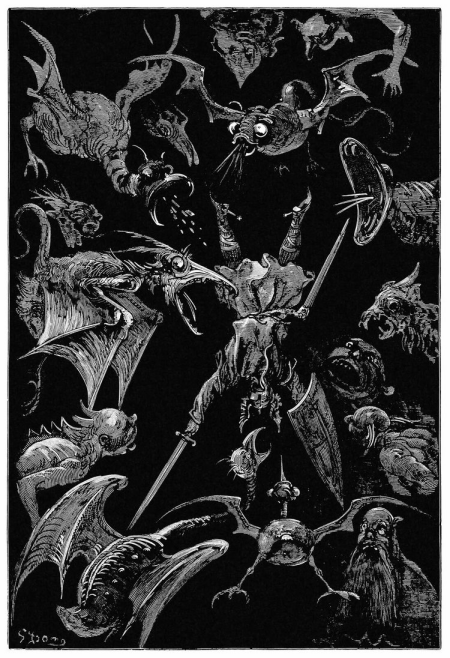
\includegraphics[scale=.5]{Horror}
  \end{center}

  \myhighlight{Amnesia}{madness-madness-amnesia}

  You forget your name, history, and background - including how to do the things detailed in your Trope, Species, or Flavor.  Put another way, you have lost the abilities that distinguish you from a peasant (though the numbers on your character sheet don't change).

  \myhighlight{Beaten}{madness-beaten}

  Your madness has left you periodically deaf and dumb to the world around you as you retreat within yourself to escape your fear. Your \mylink{Grit}{combat-flesh-grit} is 0 while under the effects of this madness and can't be healed, and you always lose Init.

  \myhighlight{Blind Fury}{madness-blind-fury}

  Your fear finds vent in violent rages and an uncontrollable temper. If provoked, you must roll \RS : \FOC.  If you fail you immediately become Enraged and execute a \mylink{Bum Rush}{combat-deeds-bum-rush} against your provoker.

  \myhighlight{Darkfear}{madness-darkfear}

  You are stuck with a permanent fear of the dark. You cannot sleep in darkness; you must have a burning candle or lamp by your side or you do not gain any of the benefits associated with a Bivouac. Additionally, whenever you are in a dark environment you take an additional -4 modifier to any \RO or \RB tries

  \myhighlight{Fanaticism}{madness-fanaticism}

  Your madness have given you the irrational belief that religious faith will protect you from your fear. All of your extra income must be spent tithing to a religious institution (you earn no Glory for money spent in this way)

  \myhighlight{Foolhardiness}{madness-foolhardiness}

  Your continued survival in the face of the unnatural has given you the irrational belief that you are invincible. You cannot retreat or withdraw from dangerous situations by any means.

  \myhighlight{Gluttony}{madness-gluttony}

  You are overcome by the irrational belief that if you consume you will not be consumed by your fear. You refuse to wear armor since it's "binding".  If you Bivouac, roll your Personal Provisions 3 times.  If you take a Vacation, your costs are increased by x3 coins (you don't receive Glory for this extra money)

  \myhighlight{Hallucinations}{madness-hallucinations}

  Unreliable senses; the Arbiter will give you false descriptions of things if you are ever alone (without your allies to guide you). Since you are always doubting your senses, you are always \mylink{Surprised}{combat-surprise} on the first round of Combat.

  \myhighlight{Melancholy}{madness-melancholy}

  You are consumed by depression and ennui. You take a -2 penalty on all \RO and \RB tries.

  \myhighlight{The Needle}{madness-the-needle}

  Only narcotics will stave off the gnawing terror. Roll a d12 on the \mylink{Narcotics}{gear-narcotics} table - you are \mylink{Addicted}{gear-narcotics-addiction} to that substance.

  \myhighlight{Night Terrors}{madness-night-terrors}

  You are unable to Bivouac unless you roll a \RS : Sanity.  Note that if you fail, it forces a roll on {Terrifying Tables}{misc-terrifying-tables}

  \myhighlight{Occult Obsession}{madness-occult-obsession}

  You are overcome with the irrational belief that if you master the occult you can master your fear. All of your extra income must be spent pursuing occult tomes and private instruction (you earn no Glory for money spent in this way)

  \myhighlight{Odious Quirks}{madness-odious-quirks}

  Your madness manifests itself as disturbing personality quirks such as talking to yourself, laughing like a maniac, saying and doing inappropriate things, etc. Your \MAX Presence is \DCDOWN x2 

  \myhighlight{Phobia}{madness-phobia}

  You are terrified of whatever thing or class of things caused this insanity.  When you encounter this trigger, you are \mylink{Afraid}{effect-afraid} for Minutes

  \myhighlight{Shot Nerves}{madness-shot-nerves}

  Your madness has weakened your already fragile mental state.  Whenever you enter Combat or a stressful situation (determined by the Arbiter), roll a \RS : \INT.  If you fail you can only stand gawping in horror for the rest of Combat.  You cannot Fight or Guard, but you can be pulled / moved by allies.

  \myhighlight{Split Personality}{madness-split-personality}

  Roll up a new level 1 character that uses your current physical stats (\VIG and \DEX), but new mental stats (\INT and \FOC). The class must be different from your current one. Each session, alternate between these two characters, each one tracking Glory separately.

  \cbreak

  \myhighlight{Starvation}{madness-starvation}

  Your madness has inspired the irrational belief that if you deny yourself food you can deny the extent of your fear. Whenever you Bivouac, roll a \RS : \FOC.  If you fail you are unable to consume your Personal Provisions (and thus get no benefit for resting).  If you Vacation while under the effect of this Madness, you start your next adventure with a maximum Flesh of 1.


  \myhighlight{True Madness}{madness-true-madness}

  Your madness is pervasive; roll twice on the Madness Effects Table and take both results. If the extent of your mental trauma is discovered, you run the risk of being institutionalized.

  \myhighlight{The Voices}{madness-the-voices}

  You are continually distracted by a number of voices that only you can hear. Whenever you roll Init, roll a \RS : \FOC.  If you fail you are \mylink{Befuddled}{effect-befuddled} for the rest of Combat. You fail all \mylink{Listen}{skill-listen} skill rolls.

  \myhighlight{Whisper of the Rapture}{madness-whisper-of-the-rapture}

  You are stuck with a permanent fear of enclosed spaces, tight fits, and premature burial. Whenever you find yourself in these circumstances suffer a -8 on all \RO and \RB tries

} %end
